\section{Results}\label{sec:results}

% ==================================================================
%
% EB writes here
%
\subsection{DINOv2 ViT}
We extracted 384 features for each of the 2061 images [camera type here], inserted them into a design matrix with rows containing a numerical feature and columns containing the image they originated from. The resulting 2961 x 384 matrix was then standardized and reduced with either PCA with 70 principal components, or UMAP with 2 embeddings. 

We present the first two components of the PCA plotted against each other in Figure \ref{fig:pca0pca1}, and the embeddings from UMAP in Figure \ref{fig:umap}. Both figures have labeled species data points, but this labels have not been provided for the DINO ViT model and are provided afterwards to see whether the feature representations we've retrieved can be considered good representations.

After analyzing the cumulative variance for each component (Appendix, Figure \ref{fig:cumsumpca}), we saw that including 70 components accounted for just above 85\% of the variance in the design matrix, and the first two components only account for around 26\%. This means that we cannot assume the PC representations to relay significant relationships in our data. 

In Figure \ref{fig:umap} we see clear clusters. We already know that the input images belonged to 14 categories, and yet we count 11 distinct cluster which is also confirmed by the silhouette score for each of the 2-20 KMeans clusters we tested (Appendix, Figure \ref{fig:kmean_sil}). We suspect that the species that have similar feature embeddings might also have some morphological similarities, which is confirmed by looking into some example photos in Figure \ref{fig:pseudo+empty}. 

\begin{figure}[H]
    \centering
    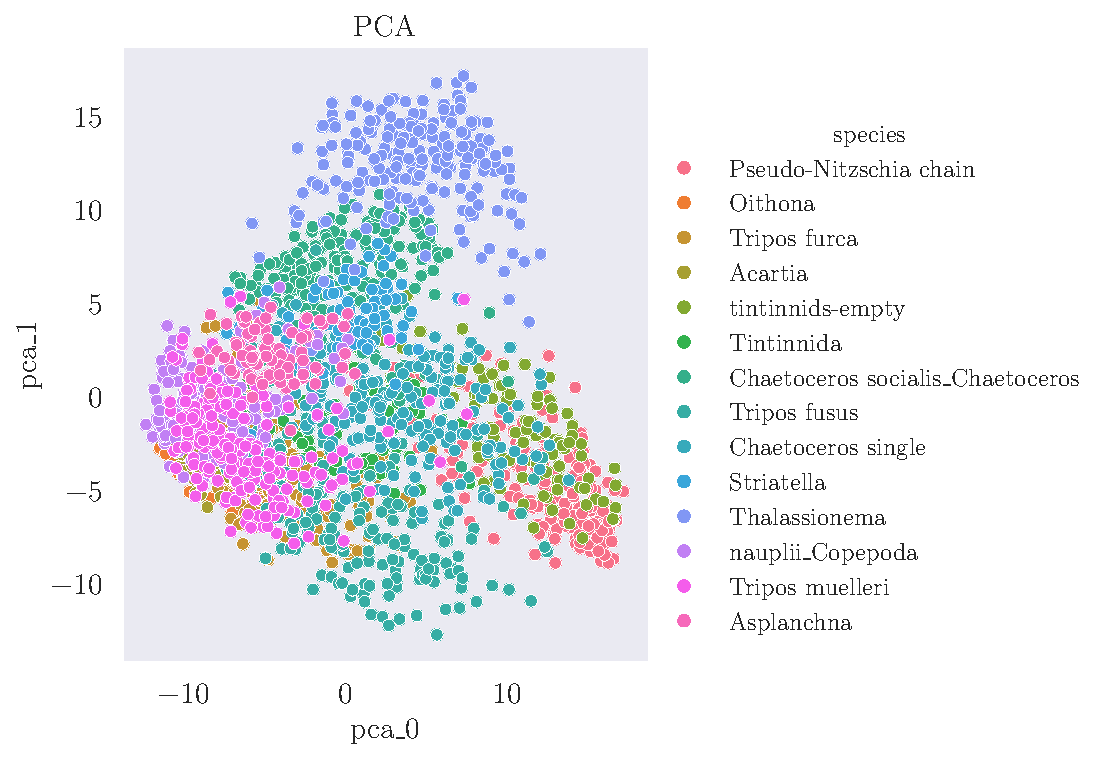
\includegraphics[width=1.1\linewidth]{examples/tests_eb/figs/pca0_pca1.pdf}
    \caption{The two first principal components out of 70 plotted against each other. Already here we can see some weak signs of clusters}
    \label{fig:pca0pca1}
\end{figure}

\begin{figure}[H]
    \centering
    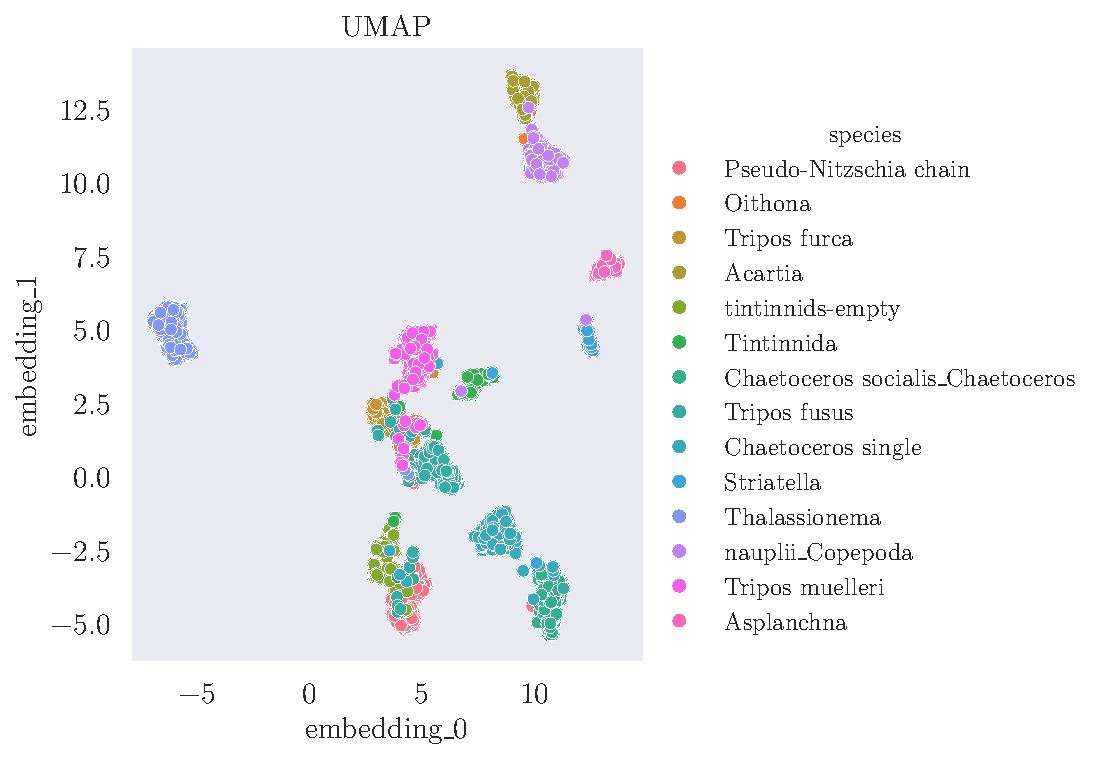
\includegraphics[width=1.1\linewidth]{examples/tests_eb/figs/umap.pdf}
    \caption{A UMAP plot to explore non-linear relations in our data (TODO - read up on UMAP). Here we can clearly see how our extracted features cluster together, yet we still do not have 14 distinct clusters.}
    \label{fig:umap}
\end{figure}

\begin{figure}[H]
    \centering
    % Første subfigur
    \begin{subfigure}[b]{0.32\linewidth}
        \centering
        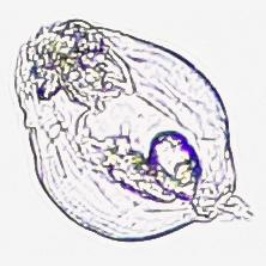
\includegraphics[width=\linewidth]{examples/tests_eb/figs/plankton_examplebatch/asplanktia.png}
        \caption{Species Asplanchna}
        \label{fig:asplanch}
    \end{subfigure}
    % Andre subfigur
    \begin{subfigure}[b]{0.32\linewidth}
        \centering
        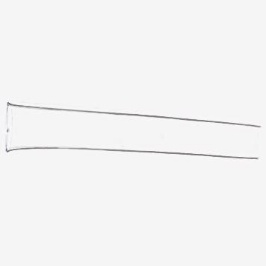
\includegraphics[width=\linewidth]{examples/tests_eb/figs/plankton_examplebatch/empty.jpg}
        \caption{Species Tintinnids-empty}
        \label{fig:empty}
    \end{subfigure}
    % Tredje subfigur
    \begin{subfigure}[b]{0.32\linewidth}
        \centering
        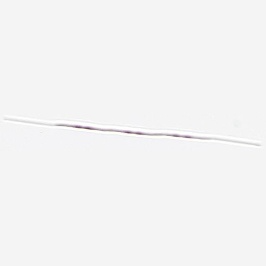
\includegraphics[width=\linewidth]{examples/tests_eb/figs/plankton_examplebatch/pseudo.png}
        \caption{Species Pseudo-Nitzschia}
        \label{fig:pseudo}
    \end{subfigure}
    \caption{In (a), we see an example of a species that has a clear, separate cluster in Figure \ref{fig:umap}. We compare this to (b) and (c), which seemingly cluster together in the same figure.}
    \label{fig:grid}
\end{figure}

Just for fun, we looked into the species that would have been misclusteded if we used KMeans clustering on the two similar species mentioned in Figure \ref{fig:grid}. 

\begin{figure}[H]
    \centering
    \begin{subfigure}[b]{1\linewidth}
        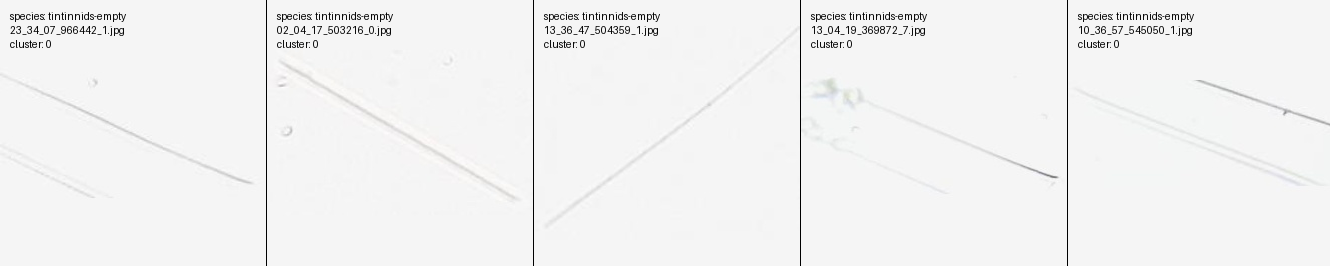
\includegraphics[width=\linewidth]{examples/tests_eb/figs/misclustered_empty.png}
        \caption{Tintinnids-empty that have clustered with Pseudo-Nitzchia chains according to simple K-means clustering of an isolated selection of UMAP embeddings for the two species.}
    \end{subfigure}
    
    \vspace{1em}
    
    \begin{subfigure}[b]{1\linewidth}
        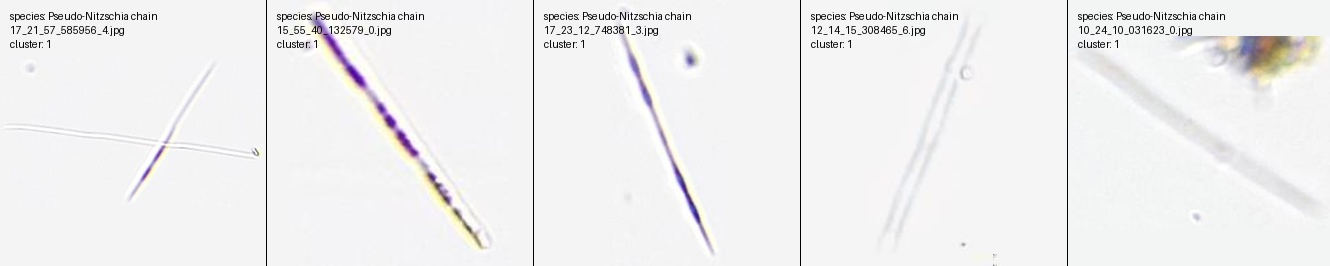
\includegraphics[width=\linewidth]{examples/tests_eb/figs/misclustered_pseudo-nitz.png}
        \caption{Pseudo-Nitzschia chains that have clustered with Tintinnids-empty according to simple K-means clustering of an isolated selection of UMAP embeddings for the two species.}
    \end{subfigure}
    \caption{We compare some of the species that seem to cluster together in Figure \ref{fig:umap} to explore whether the original labels are incorrect or if our DINOv2 fails to discern between the two species. The clustering process demonstrated in Figure \ref{fig:misclustering_process} in our Appendix.}
    \label{fig:misclusters}
\end{figure}


% ==================================================================